%%%%%%%%%%%%%%%%%%%%%%%%%%%%%%%%%%%%%%%%%%%%%%%%%%%%%%%%%%%%%%%%%%%%%%%%%%%%%%%%%%%%%%%%%%%%%
%%									ANNEXES 												%
%%%%%%%%%%%%%%%%%%%%%%%%%%%%%%%%%%%%%%%%%%%%%%%%%%%%%%%%%%%%%%%%%%%%%%%%%%%%%%%%%%%%%%%%%%%%%
\chapter{Annexes}

%%%%%%%%%%%%%%%%%%%%%%%%%%%%%%%%%%%%%%%%%%%%%%%%%%%%%%%%%%%%%%%%%%%%%%%%%%%%%%%%%%%%%%%%%%%%%


\section{Figures annexes}
	\blindtext
	On rappelle que \gls{alpha} et \gls{gamma} sont liés par la relation~\eqref{eq:alphagamma}. Pour plus de détails, voir page~\pageref{eq:alphagamma}.
	
\begin{figure}[!h]
	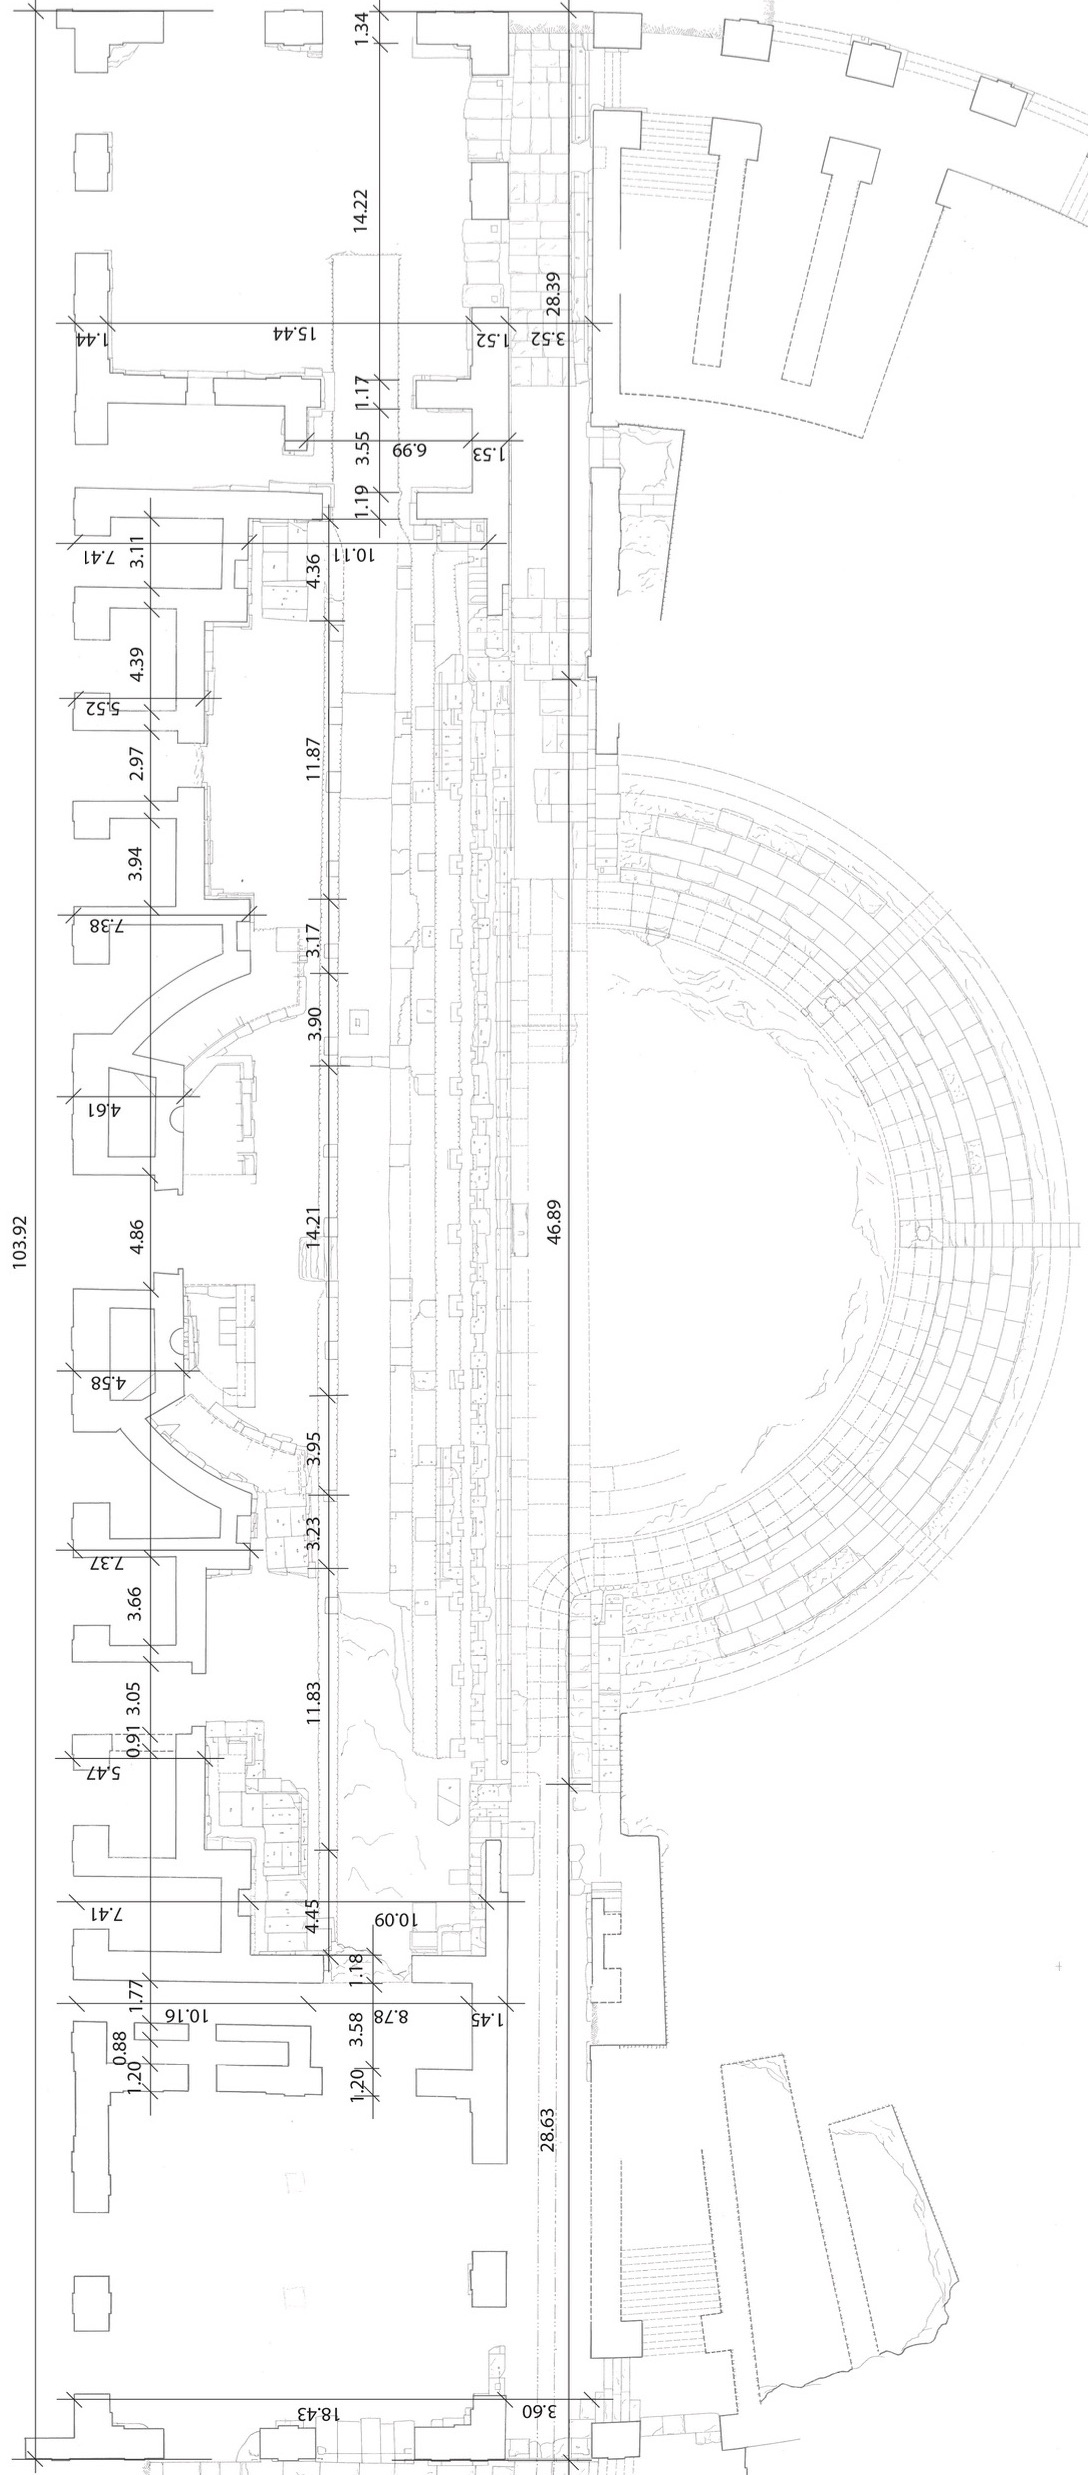
\includegraphics[height=0.8\paperheight]{images/cotes}
	\caption[Plan du rez-de-chaussée au bâtiment de scène]{Plan du rez-de-chaussée au bâtiment de scène \cite[Pl. XXI]{orangePl}}
	\label{cotes} 
\end{figure} 
	

\section{Tableaux annexes}
	\blindtext